
% This LaTeX was auto-generated from an M-file by MATLAB.
% To make changes, update the M-file and republish this document.

\documentclass{article}
\usepackage{graphicx}
\usepackage{color}
\usepackage{listings}
\usepackage[framed]{mcode}
\usepackage{fullpage}
\usepackage{amsmath}
\usepackage[utf8x]{inputenc}
\usepackage{import}
\usepackage{setspace}
\usepackage{hyperref}
\definecolor{lightgray}{gray}{0.5}
\setlength{\parindent}{0pt}

\begin{document}

    
    
%\section*{}

 \title{BE 521: Homework 4 \\{\normalsize HFOs}
\\{\normalsize Spring 2021}} \author{58 points} \date{Due: Tuesday,
2/23/2021 10:00pm} \maketitle \textbf{Objective:} HFO detection and
cross-validation 
 \begin{center} \author{Jal Mahendra Panchal \\
  \normalsize Collaborators: COLLABORATORS HERE \\}
\end{center}


\subsection*{HFO Dataset} High frequency oscillations (HFOs) are
quasi-periodic intracranial EEG transients with durations on the
order of tens of milliseconds and peak frequencies in the range of
80 to 500 Hz. There has been considerable interest among the
epilepsy research community in the potential of these signals as
biomarkers for epileptogenic networks.\\\\
In this homework exercise, you will explore a dataset of candidate
HFOs detected using the algorithm of Staba et al. (see article on
Canvas). The raw recordings from which this dataset arises come from
a human subject with mesial temporal lobe epilepsy and were
contributed by the laboratory of Dr. Greg Worrell at the Mayo Clinic
in Rochester, MN.\\\\
The dataset \verb|I521_A0004_D001| contains raw HFO clips that are
normalized to zero mean and unit standard deviation but are
otherwise unprocessed. The raw dataset contain two channels of data:
\verb|Test_raw_norm| and \verb|Train_raw_norm|, storing raw testing
and training sets of HFO clips respectively. The raw dataset also
contains two annotation layers: \verb|Testing windows| and
\verb|Training windows|, storing HFO clip start and stop times (in
microseconds) for each of the two channels above.
Annotations contain the classification by an ``expert'' reviewer
(i.e., a doctor) of each candidate HFO as either an HFO (2) or an
artifact (1). On ieeg.org and upon downloading the annotations,
You can view this in the "description" field. \\\\
After loading the dataset in to a \verb|session| variable as in
prior assignments you will want to familiarize yourself with the
\verb|IEEGAnnotationLayer| class. Use the provided "getAnnotations.m"
function to get all the annotations from a given dataset. The first
output will be an array of annotation objects, which you will see
also has multiple fields including a description field as well as start and stop times. Use
You can use the information outputted by getAnnotations to pull
each HFO clip.


\section{Simulating the Staba Detector (12 pts)} Candidate HFO clips
were detected with the Staba et al. algorithm and subsequently
validated by an expert as a true HFO or not. In this first section,
we will use the original iEEG clips containing HFOs and re-simulate
a portion of the Staba detection.
\begin{enumerate}
    \item How many samples exist for each class (HFO vs artifact) in
    the training set? (Show code to support your answer) (1 pt).\\


\textbf{Answer 1.1:}

\begin{lstlisting}
%Fetch I521_A0004_D001 data
addpath(genpath('/Users/jalpanchal/git/be521'));

session_hfo = IEEGSession('I521_A0004_D001', 'jalpanchal', 'jal_ieeglogin.bin');
sampling_frequency_hz_hfo = session_hfo.data.sampleRate;
duration_in_sec_hfo = session_hfo.data(1).rawChannels(1).get_tsdetails.getDuration/1e6;

test_raw_norm = session_hfo.data.getvalues(0, duration_in_sec_hfo * 1e6, 1);
train_raw_norm = session_hfo.data.getvalues(0, duration_in_sec_hfo * 1e6, 2);

datestr(seconds(duration_in_sec_hfo),'HH:MM:SS:FFF')
\end{lstlisting}

\color{lightgray} \begin{lstlisting}IEEGSETUP: Adding 'ieeg-matlab.jar' to dynamic classpath
Warning: Objects of edu/upenn/cis/db/mefview/services/TimeSeriesDetails
class exist - not clearing java 
Warning: Objects of edu/upenn/cis/db/mefview/services/TimeSeriesInterface
class exist - not clearing java 
IEEGSETUP: Found log4j on Java classpath.
URL: https://www.ieeg.org/services
Client user: jalpanchal
Client password: ****

ans =

    '00:00:09:466'

\end{lstlisting} \color{black}
\begin{lstlisting}
%Get annotations
dataset = session_hfo.data;
layerName = 'Training windows';
[allEvents, timesUSec, channels] = getAnnotations(dataset,layerName);
\end{lstlisting}
\begin{lstlisting}
%parsing description and event timing
events_train = [str2double(allEvents(1).description), allEvents(1).start,...
               allEvents(1).stop ];
for i = 2:size(allEvents,2)
    events_train = [events_train;str2double(allEvents(i).description),...
        allEvents(i).start, allEvents(i).stop];
end
\end{lstlisting}
\begin{lstlisting}
hfo_train = find(events_train(:, 1)==2);
artif_train = find(events_train(:, 1)==1);

number_hfo_training = size(hfo_train, 1)
number_artifact_training =  size(artif_train,1)
\end{lstlisting}

\color{lightgray} \begin{lstlisting}
number_hfo_training =

   101


number_artifact_training =

    99

\end{lstlisting} \color{black}
The number of samples for HFo are 101 and that for artifacts are 99.

    \item Using the training set, find the first occurrence of the
    first valid HFO and the first artifact.
        Using \verb|subplot| with 2 plots, plot the valid HFO's
        (left) and artifact's (right) waveforms. Since the units are
        normalized, there's no need for a y-axis, so remove it with
        the command \verb|set(gca,'YTick',[])|. (2 pts).\\


\textbf{Answer 1.2:}

\begin{lstlisting}
%test_raw_norm = session_hfo.data.getvalues(0, duration_in_sec_hfo * 1e6, 1);
%fetching first occurance of HFO
fs = sampling_frequency_hz_hfo;
t_hfo = events_train(hfo_train(1),2)/1e3 : 1e3/fs : events_train(hfo_train(1),3)/1e3;
hfo_1_train = session_hfo.data.getvalues(events_train(hfo_train(1),2), events_train(hfo_train(1),3)-events_train(hfo_train(1),2), 2);

%fetching first occurance of artifact
t_artif = events_train(artif_train(1),2)/1e3 : 1e3/fs : events_train(artif_train(1),3)/1e3;
artif_1_train = session_hfo.data.getvalues(events_train(artif_train(1),2), events_train(artif_train(1),3)-events_train(artif_train(1),2), 2);
\end{lstlisting}
\begin{lstlisting}
%plots
figure();
ax1 = subplot(1,2,1);
plot(t_hfo, hfo_1_train, 'Linewidth', 2);
title('HFO(1)')
xlabel('Time (ms)')
set(ax1, 'YTick', [])
ax1.Position = [0.1300 0.1100 0.3747 0.8150];

ax2 = subplot(1,2,2);
plot(t_artif, artif_1_train, 'Linewidth', 2)
title('Artifact(1)')
xlabel('Time (ms)')
set(ax2, 'YTick', [])
ax2.Position = [0.5303 0.1100 0.3747 0.8150];


suptitle('First samples in training window in I521\_A0004\_D001')
\end{lstlisting}


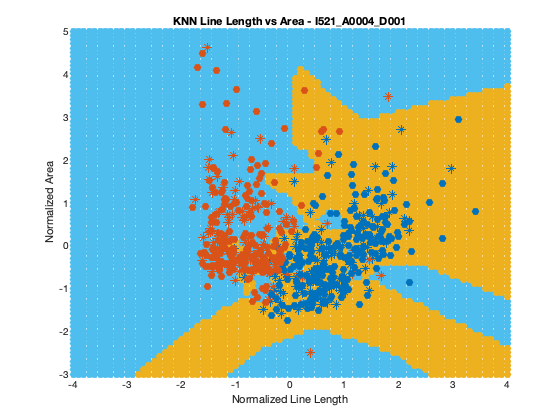
\includegraphics [width=5in]{jalp_hw4_01.png}

    \item Using the \texttt{fdatool} in MATLAB, build an FIR
    bandpass filter of the equiripple type of order 100.
        Use the Staba et al. (2002) article to guide your choice of
        passband and stopband frequency. Once set, go to
        \texttt{File} \verb|->| \texttt{Export}, and export
        ``Coefficients'' as a MAT-File. Attach a screenshot of your
        filter's magnitude response. (Note: We will be flexible with
        the choice of frequency parameters within reason.) (3 pts) \\


\textbf{Answer 1.3:}


    \item Using the forward-backward filter function
    (\texttt{filtfilt}) and the numerator coefficients saved above,
        filter the valid HFO and artifact clips obtained earlier.
        You will need to make a decision about the input argument
        \texttt{a} in the \texttt{filtfilt} function. Plot these two
        filtered clips overlayed on their original signal in a two
        plot \texttt{subplot} as before. Remember to remove the
        y-axis. (3 pts) \\


\textbf{Answer 1.4:}


    \item Speculate how processing the data using Staba's method may
    have erroneously led to a false HFO detection (3 pts) \\


\textbf{Answer 1.5:}


\end{enumerate}
\section{Defining Features for HFOs (9 pts)} In this section we will
be defining a feature space for the iEEG containing HFOs and
artifacts. These features will describe certain attributes about the
waveforms upon which a variety of classification tools will be
applied to better segregate HFOs and artifacts
\begin{enumerate}
    \item Create two new matrices, \verb|trainFeats| and
    \verb|testFeats|, such that the number of rows correspond to
    observations (i.e. number of training and testing clips)
        and the number of columns is two. Extract the line-length and
        area features (seen previously in lecture and Homework 3) from
        the normalized raw signals (note: use the raw signal from
        ieeg.org, do not filter the signal). Store the line-length value
        in the first column and area value for each sample in the second
        column of your features matrices. Make a scatter plot of the
        training data in the 2-dimensional feature space, coloring the
        valid detections blue and the artifacts red. (Note: Since we only
        want one value for each feature of each clip, you will
        effectively treat the entire clip as the one and only
        ``window''.) (4 pts) \\


\textbf{Answer 2.1:}


    \item Feature normalization is often important. One simple
    normalization method is to subtract each feature by its mean and
    then divide by its standard deviation
        (creating features with zero mean and unit variance). Using
        the means and standard deviations calculated in your
        \emph{training} set features, normalize both the training
        and testing sets. You should use these normalized features for
        the remainder of the assignment.
    \begin{enumerate} \item What is the statistical term for the
    normalized value, which you have just computed? (1 pt) \\


\textbf{Answer 2.2a:}


	\item Explain why such a feature normalization might be critical
	to the performance of a $k$-NN classifier. (2 pts) \\


\textbf{Answer 2.2b:}


\item Explain why (philosophically) you use the training feature means and
	standard deviations to normalize the testing set. (2 pts) \\


\textbf{Answer 2.2c:}


    \end{enumerate}
\end{enumerate}
\section{Comparing Classifiers (20 pts)} In this section, you will
explore how well a few standard classifiers perform on this dataset.
Note, the logistic regression, $k$-NN, and SVM classifiers are functions
built into some of Matlabs statistics packages. If you don't have
these (i.e., Matlab doesn't recognize the functions), and you are
experiencing any difficulty downloading the necessary packages, please
let us know.
\begin{enumerate}
 \item Using Matlab's logistic regression classifier function,
 (\texttt{mnrfit}), and its default parameters, train a model on the
 training set. Using Matlab's \texttt{mnrval} function, calculate
 the training error (as a percentage) on the data. For extracting
 labels from the matrix of class probabilities, you may find the
 command \texttt{[$\sim$,Ypred] = max(X,[],2)} useful\footnote{Note:
 some earlier versions of Matlab don't like the \texttt{$\sim$},
 which discards an argument, so just use something like
 \texttt{[trash,Ypred] = max(X,[],2)} instead.}, which gets the
 column-index of the maximum value in each row (i.e., the class with
 the highest predicted probability). (3 pts) \\


\textbf{Answer 3.1:}


 \item Using the model trained on the training data, predict the
 labels of the test samples and calculate the testing error. Is the
 testing error larger or smaller than the training error? Give one
 sentence explaining why this might be so. (2 pts) \\


\textbf{Answer 3.2:}


 \item
  \begin{enumerate}
   \item Use Matlab's $k$-nearest neighbors function,
   \texttt{fitcknn}, and its default parameters ($k$ = 1, among
   other things), calculate the training and testing errors. (3 pts) \\


\textbf{Answer 3.3a:}


   \item Why is the training error zero? (2 pts) \\


\textbf{Answer 3.3b:}


  \end{enumerate}
 \item Now, train Matlab's implementation of a
 support vector machine (SVM), \texttt{fitcsvm}. Report the training and testing
 errors for an SVM model with a radial basis function (RBF) kernel function,
 while keeping other parameters at their default values. (3 pts) \\


\textbf{Answer 3.4 :}


 \item It is sometimes useful to visualize the decision boundary of
 a classifier. To do this, we'll plot the classifier's prediction
 value at every point in the ``decision'' space. Use the
 \texttt{meshgrid} function to generate points in the line-length
 and area 2D feature space and a scatter plot (with the \verb|'.'|
 point marker) to visualize the classifier decisions at each point
 (use yellow and cyan for your colors). In the same plot, show the
 training samples (plotted with the '*' marker to make them more
 visible) as well. As before use blue for the valid detections and
 red for the artifacts. Use ranges of the features that encompass
 all the training points and a density that yields that is
 sufficiently high to make the decision boundaries clear. Make such
 a plot for the logistic regression, $k$-NN, and SVM classifiers. (4
 pts) \\


\textbf{Answer 3.5:}


 \item In a few sentences, report some observations about the three
 plots, especially similarities and differences between them. Which
 of these has overfit the data the most? Which has underfit the data
 the most? (3 pts) \\


\textbf{Answer 3.6:}


\end{enumerate}
\section{Cross-Validation (17 pts)} In this section, you will
investigate the importance of cross-validation, which is essential
for choosing the tunable parameters of a model (as opposed to the
internal parameters the the classifier ``learns'' by itself on the
training data).
\begin{enumerate}
 \item Since you cannot do any validation on the testing set, you'll
 have to split up the training set. One way of doing this is to
 randomly split it into $k$ unique ``folds,'' with roughly the same
 number of samples ($n/k$ for $n$ total training samples) in each
 fold, training on $k-1$ of the folds and doing predictions on the
 remaining one.
 In this section, you will do 10-fold cross-validation, so create a
 cell array\footnote{A cell array is slightly different from a
 normal Matlab numeric array in that it can hold elements of
 variable size (and type), for example \texttt{folds\{1\} = [1 3 6]; folds\{2\}
 = [2 5]; folds\{3\} = [4 7];}.} \texttt{folds} that contains 10
 elements, each of which is itself an array of the indices of
 training samples in that fold. You may find the \texttt{randperm}
 function useful for this.
 Using the command \texttt{length(unique([folds\{:\}]))}, show that
 you have 200 unique sample indices (i.e. there are no repeats
 between folds). (2 pts) \\


\textbf{Answer 4.1:}


 \item Train a new $k$-NN model (still using the default parameters)
 on the folds you just created. Predict the labels for each fold
 using a classifier trained on all the other folds. After running
 through all the folds, you will have label predictions for each
 training sample.
  \begin{enumerate}
   \item Compute the error (called the validation error) of these
   predictions. (3 pts) \\


\textbf{Answer 4.2a:}


\item How does this error compare (lower,
   higher, the same?) to the error you found in question 3.3? Does
   it make sense? (2 pts) \\


\textbf{Answer 4.2b:}


  \end{enumerate}
 \item Create a parameter space for your $k$-NN model by setting a
 vector of possible $k$ values from 1 to 30. For each values of $k$,
 calculate the validation error and average training error over the
 10 folds.
  \begin{enumerate}
   \item Plot the training and validation error values over the
   values of $k$, using the formatting string \texttt{'b-o'} for the
   validation error and \texttt{'r-o'} for the training error. (4
   pts) \\


\textbf{Answer 4.3a:}


\item What is the optimal $k$ value and its training and testing error?
(1 pts) \\


\textbf{Answer 4.3b:}


   \item Explain why $k$-NN generally overfits less with higher
   values of $k$. (2 pts) \\


\textbf{Answer 4.3c:}


  \end{enumerate}
 \item
  \begin{enumerate}
   \item Using your optimal value for $k$ from CV, calculate the
   $k$-NN model's \textit{testing} error. (1 pts) \\


\textbf{Answer 4.4a:}


\item How does this
   model's testing error compare to the $k$-NN model
   you trained in question 3.3? Is it the best of the three models
   you trained in Section 3? (2 pts) \\


\textbf{Answer 4.4b:}


  \end{enumerate}
\end{enumerate}




\end{document}
    
